\chapter{Aprendizado não supervisionado}

\framebox[\textwidth]{
	\hspace{1em}
	\vbox{
		\textbf{Leitura obrigatória:}
		\begin{itemize}
			\item \cite{FaceliEtAl2011} -- Cap. 11 (Análise de agrupamentos).
			\item \cite{FaceliEtAl2011} -- Cap. 11 (Algoritmos de agrupamentos).
		\end{itemize}
		
		\textbf{Leitura complementar:}
		\begin{itemize}
			\item \cite{MullerAndGuido2017} -- Cap. 3 (Unsupervised Learning and Preprocessing).
		\end{itemize}
	}
}

\section{Visão geral}

Conforme apresentado no Capítulo~\ref{cap:conceitos-basicos-aprendizagem-maquina}, métodos não supervisionados de aprendizagem de máquina extraem características das instâncias sem a necessidade de estarem rotuladas. Por conta disso, estes métodos são classificados como \textit{descritivos}. Uma das tarefas às quais se aplicam é o \textbf{agrupamento}, que tem por objetivo formar grupos com dados similares entre si. A Figura~\ref{fig:exemplos-agrupamentos} apresenta alguns exemplos de agrupamento. O primeiro quadro (superior esquerdo) apresenta um conjunto de objetos. Estes objetos podem ser agrupados segundo diferentes aspectos. O segundo quadro (superior direito) agrupa os objetos segundo sua forma, enquanto o terceiro quadro (inferior esquerdo) agrupa segundo o preenchimento de cada objeto. Finalmente, os objetos podem ser agrupados considerando os dois aspectos (formato e preenchimento) simultaneamente, o que é apresentado no quarto quadro (inferior direito).

\begin{figure}
	\centering
	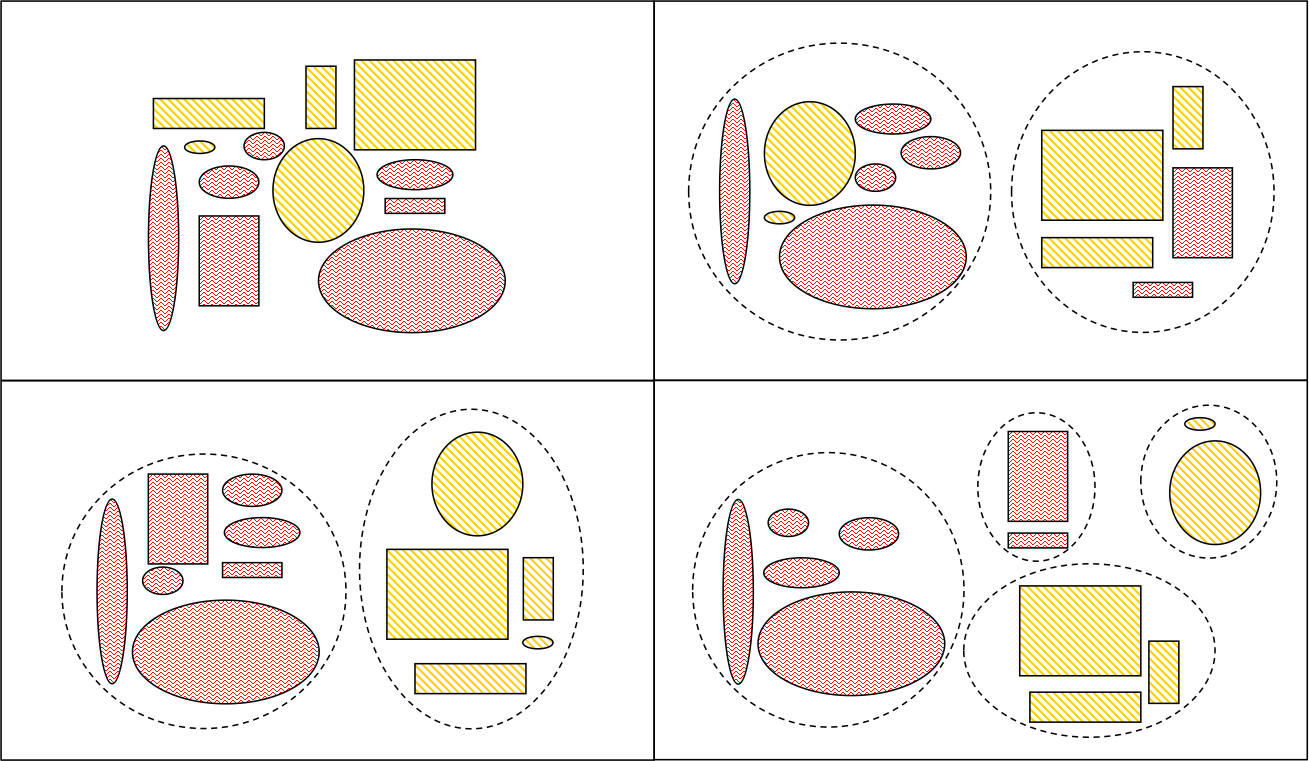
\includegraphics[width=0.7\textwidth]{img/exemplos-agrupamentos}
	\caption{Exemplos de possíveis agrupamentos de um conjunto de objetos}
	\label{fig:exemplos-agrupamentos}
\end{figure}

Uma aplicação típica das técnicas de agrupamento é a identificação de perfis similares de consumidores. Por exemplo, pode ser útil determinar consumidores com gostos em comum no serviço \textit{Netflix}. Ao agrupar os usuários de acordo com seus gostos, é possível direcionar a apresentação de novos títulos em função dessa informação. Se em um grupo de usuários com gostos similares, metade deles avaliou bem um determinado título, seria interessante apresentar este título aos usuários que ainda não assistiram, pois a probabilidade de aceitação é alta. Um segundo exemplo acontece nos mecanismos de busca da Internet. Dado o histórico de visitas de um usuário, quando ele realiza uma nova pesquisa, o motor de busca agrupa os resultados pela similaridade com seu histórico, apresentando assim resultados que com maior probabilidade interesse ao usuário.

Existem diferentes estratégias para agrupamento, como abordagens baseadas em proximidade, probabilísticas ou baseadas em hierarquia. Este capítulo apresenta dois algoritmos de agrupamento, um hierárquico e outro particional. O \textbf{algoritmo hierárquico aglomerativo} é um método que cria diferentes grupos de dados em uma estrutura de hierarquia, que pode ser decomposta conforme a hierarquia desejada. O algoritmo \textbf{$K$-Means} (ou $K$-Médias) é um método particional baseado na proximidade dos dados que utiliza um conjunto de centroides para definir cada grupo.

Ambos os métodos exigem a definição das métricas de similaridade entre dois indivíduos do conjunto de dados. Conforme apresentado no Capítulo~\ref{cap:aprendizado-supervisionado}, uma métrica muito comum é a distância Euclidiana. Seja $x_i$ o valor do atributo $i$ do objeto $x$ e $d$ o número de atributos do objeto, a distância entre dois objetos $a$ e $b$ pode ser definida como:

$$
d(a, b) = \sqrt{\sum_{i=1}^{d} (a_i - b_i)^2}
$$

Para atributos qualitativos, podemos definir que a distância entre dois objetos $a$ e $b$ em função do atributo $i$ (portanto $a_i - b_i$) é 1, caso $a_i \neq b_i$ e 0, caso $a_i = b_i$. Com isso, podemos calcular a distância total em função de todos os $d$ atributos qualitativos como:

$$
d(a, b) = \sum_{i=1}^{d} (a_i - b_i)
$$

Com isso, se um conjunto de dados possui tanto atributos quantitativos quanto qualitativos, devemos calcular as duas distâncias (utilizando os dois conjuntos de atributos) e somá-las para obter a distância final. As seções seguintes apresentam em detalhes o agrupamento de dados utilizando estas métricas de distância.

\section{Agrupamento particional}

Os métodos particionais de agrupamento criam um conjunto de \textit{clusters} (grupos) iniciais e, iterativamente, movem elementos de um \textit{cluster} a outro a fim de melhorar o valor do critério de agrupamento. O número de \textit{clusters} é um parâmetro fixo do algoritmo e um critério comum de agrupamento é a distância entre cada elemento e o centroide do \textit{cluster} ao qual pertence.

\subsection{Algoritmo de \textit{K}-Means}

O principal método de agrupamento particional é o $K$-Means (ou $K$-Médias), que é também um dos algoritmos de agrupamento mais simples e conhecidos. Seu pseudocódigo é apresentado no Algoritmo~\ref{alg:k-means}. O algoritmo escolhe aleatoriamente $k$ objetos do conjunto de dados para formarem os centroides dos $k$ \textit{clusters} que serão construídos. Iterativamente, para cada objeto calcula-se a distância para cada um dos $k$ centroides. O objeto é alocado ao \textit{cluster} cujo centroide está mais próximo. Quando todos os objetos foram alocados, os centroides são recalculados. Na iteração seguinte, os centroides já foram recalculados e alguns objetos passam a estar mais próximo de outro centroide. Neste caso, estes objetos são realocados e os centroides são recalculados. O algoritmo termina quando não existe mais movimentação de objetos de um centroide a outro. Ao final, cada objeto pertence a um dos $k$ \textit{clusters}.

\begin{algorithm}[h]
	\DontPrintSemicolon
	\Entrada{\textit{conjunto de dados -- $X$, número de clusters $k$}}
	\Saida{\textit{partição de $X$ em $k$ clusters}}
	
	\Inicio{
		Escolhe aleatoriamente $k$ elementos de $X$ para formarem os centroides dos \textit{clusters}\;
		
		\Repita{não haverem mais objetos a serem alterados de cluster}{
			\Para{cada objeto $x_i \in X$}{
				\Para{cada cluster $C_j, j = 1, \hdots, k$}{
					Calcula distância entre o objeto $x$ e o centroide $\overline{c}_j$ do cluster $C_j$\;
				}
				Associa $x_i$ ao \textit{cluster} com centroide mais próximo\;
			}
			
			\Para{cada cluster $C_j, j = 1, \hdots, k$}{
				Recalcula o centroide\;
			}
		}
	}
	
	\caption{Pseudocódigo para o algoritmo $K$-Means}
	\label{alg:k-means}
\end{algorithm}

O cálculo do centroide é bastante simples: para cada atributo, o centroide apresenta o valor médio do atributo nos objetos pertencente a ele. No caso de atributos qualitativos, o centroide apresenta a moda observada nos objetos pertencentes a ele. Pelo fato do algoritmo se basear na distância entre os objetos e os centroides, os \textit{clusters} formados são compactos e possuem formato esférico.

Entre as limitações do $K$-Means, destacam-se o fato de não se ajustar a \textit{clusters} com formatos irregulares e a necessidade do usuário informar o número de \textit{clusters}. Para muitos problemas, não se conhece o valor adequado de $k$, o que influencia diretamente na qualidade do agrupamento. Existem algumas variantes deste algoritmo que buscam minimizar estes problemas. A principal vantagem deste algoritmo é sua baixa complexidade -- $O(n)$ -- uma vez que o número de iterações é tipicamente pequeno, $k << n$ e $d << n$.

\begin{figure}[h]
	\centering
	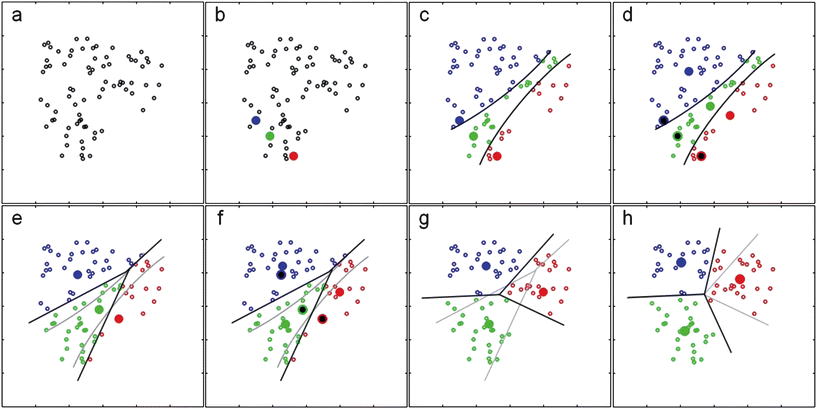
\includegraphics[width=\textwidth]{img/funcionamento-k-means}
	\caption{Funcionamento do algoritmo $K$-Means}
	\label{fig:funcionamento-k-means}
\end{figure}

A Figura~\ref{fig:funcionamento-k-means} apresenta o funcionamento do $K$-Means para um conjunto de dados de duas dimensões. No passo \texttt{(a)} são apresentados os dados, posicionados em função dos valores dos seus dois atributos. No passo \texttt{(b)} são escolhidos três pontos como os centroides (nas cores azul, verde e vermelho), portanto $k = 3$ (existem 3 \textit{clusters}). Os elementos são alocados aos \textit{clusters} no passo \texttt{(c)}. No passo \texttt{(d)}, os centroides são recalculados em função dos elementos dos seu \textit{cluster}. Com isso, os elementos são realocados no passo \texttt{(e)}. O processo se repete nos passos seguintes até a convergência. A figura ainda apresenta as fronteiras que dividem cada \textit{cluster}, conforme a posição dos seus centroides.

\subsection{Exemplo -- agrupamento particional de alunos}
\label{sec:exemplo-k-means}

Vamos considerar um conjunto de dados contendo as notas obtidas por cinco alunos ($A_1, \hdots, A_5$) nas disciplinas de português e matemática. A Tabela~\ref{tab:dados-notas-alunos} apresenta os valores para este conjunto de dados. A Figura~\ref{fig:dados-notas-alunos} apresenta uma representação gráfica destes dados.

\begin{table}[h]
	\centering
	
	\begin{tabular}{lrr}
		\hline
		\textbf{Aluno} & \textbf{Português} & \textbf{Matemática} \\
		\hline
		$A_1$ & 7,0 & 6,5 \\
		$A_2$ & 2,0 & 3,0 \\
		$A_3$ & 7,0 & 5,0 \\
		$A_4$ & 9,5 & 8,0 \\
		$A_5$ & 3,0 & 2,0 \\
		\hline
	\end{tabular}
	
	\caption{Conjunto de dados das notas dos alunos}
	\label{tab:dados-notas-alunos}
\end{table}

\begin{figure}[h]
	\centering
	\pgfplotsset{cycle list={black}}
	
	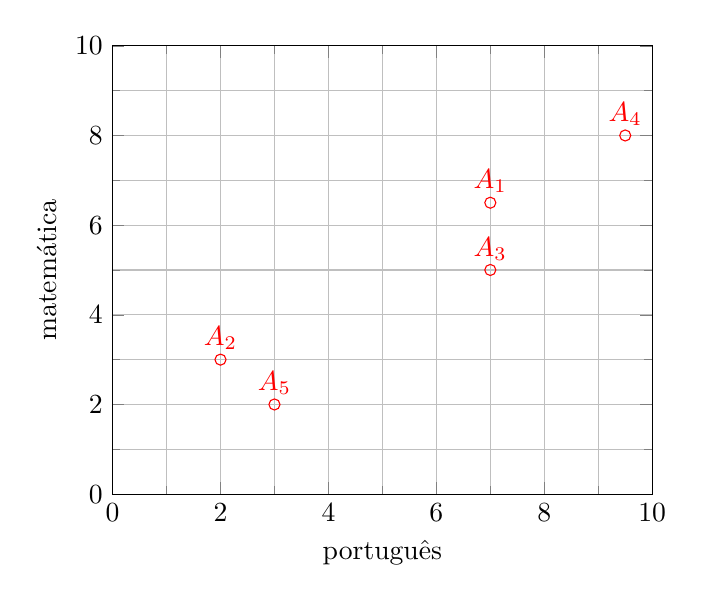
\begin{tikzpicture}
		\begin{axis}[
			grid=both,
			xmin=0, xmax=10,
			ymin=0, ymax=10,
			minor tick num = 1,
			nodes near coords,
			xlabel=português,
			ylabel=matemática
		]
		
			\addplot+[only marks, point meta=explicit symbolic, mark=o]
				coordinates {
				(7, 6.5) [$A_1$]
				(2, 3) [$A_2$]
				(7, 5) [$A_3$]
				(9.5, 8) [$A_4$]
				(3, 2) [$A_5$]
			};
		\end{axis}
	\end{tikzpicture}
	
	\caption{Representação gráfica das notas dos alunos}
	\label{fig:dados-notas-alunos}
\end{figure}

O primeiro passo consiste em definir o número de \textit{clusters} desejado $k$. Para este exemplo, consideremos $k = 2$. Com isso, definimos aleatoriamente dois elementos para servirem de centroides iniciais. Consideremos os elementos $A_1$ e $A_3$ como centroides e, portanto, $\overline{c}_1 = (7,0; 6,5)$ e $\overline{c}_2 = (7,0; 5,0)$. A Figura~\ref{fig:dados-notas-alunos-centroides-iniciais} apresenta os dados com os centroides posicionados em $A_1$ e $A_3$.

\begin{figure}[h]
	\centering
	\pgfplotsset{cycle list={black\\red\\blue\\}}
	
	
	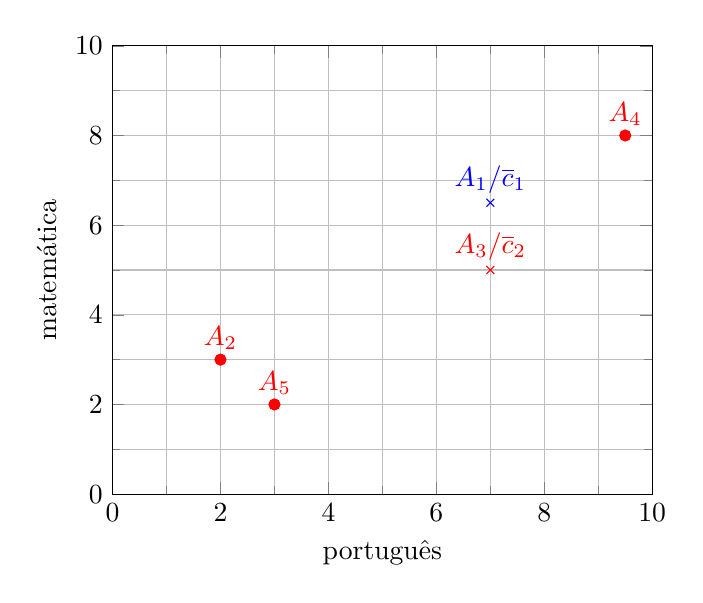
\begin{tikzpicture}
	\begin{axis}[
		grid=both,
		xmin=0, xmax=10,
		ymin=0, ymax=10,
		minor tick num = 1,
		nodes near coords,
		xlabel=português,
		ylabel=matemática
	]
	
	\addplot+[only marks, point meta=explicit symbolic, mark=*]
		coordinates {
			(2, 3) [$A_2$]
			(9.5, 8) [$A_4$]
			(3, 2) [$A_5$]
		};
		
	\addplot+[only marks, point meta=explicit symbolic, mark=x]
		coordinates {
			(7, 6.5) [$A_1$/$\overline{c}_1$]
		};
	
	\addplot+[only marks, point meta=explicit symbolic, mark=x]
		coordinates {
			(7, 5) [$A_3$/$\overline{c}_2$]
		};
	\end{axis}
	\end{tikzpicture}
	
	\caption{Representação gráfica das notas dos alunos com centroides iniciais}
	\label{fig:dados-notas-alunos-centroides-iniciais}
\end{figure}

O passo seguinte é calcular as distâncias de cada ponto para cada centroide. A métrica adotada é a distância euclidiana. Logo, podemos calcular a distância entre o ponto $A_2$ e o centroide $\overline{c}_1$ como:

\begin{align*}
d(A_2, \overline{c}_1) &= \sqrt{\sum_{i=1}^{d} ({A_2}_i - {\overline{c}_1}_i)^2} \\[10pt]
&= \sqrt{(2,0 - 7,0)^2 + (3,0 - 6,5)^2} \\[10pt]
&= \sqrt{(-5,0)^2 + (-3,5)^2} \\[10pt]
&= \sqrt{25 + 12,25} \\[10pt]
&= \sqrt{37,25} \\[10pt]
&= 6,1
\end{align*}

A matriz de distâncias entre cada elemento e cada centroide é:

\insertspace

\begin{center}
	\begin{tabular}{cccccccc}
		& & $A_1$ & $A_2$ & $A_3$ & $A_4$ & $A_5$ & \\
		$\overline{c}_1$ & \multirow{2}{*}{$\Bigg[$} & 0,0  & 6,1  & 1,5  & 2,9  & 6,0  & \multirow{2}{*}{$\Bigg]$} \\
		\multicolumn{1}{l}{$\overline{c}_2$} & & 1,5  & 5,4  & 0,0  & 3,9  & 5,0  &                  
	\end{tabular}
\end{center}

\insertspace

Com base na matriz de distâncias, atribuímos cada elemento a um dos \textit{clusters}. Caso ele esteja mais próximo do centroide $\overline{c}_1$, ele é alocado ao primeiro \textit{cluster}. Caso ele esteja mais próximo do centroide $\overline{c}_2$, ele é alocado ao segundo \textit{cluster}. A alocação resultante é (matriz de alocação):

\insertspace

\begin{center}
	\begin{tabular}{cccccccc}
		& & $A_1$ & $A_2$ & $A_3$ & $A_4$ & $A_5$ & \\
		$\overline{c}_1$ & \multirow{2}{*}{$\Bigg[$} & 1  & 0  & 0  & 1  & 0  & \multirow{2}{*}{$\Bigg]$} \\
		\multicolumn{1}{l}{$\overline{c}_2$} & & 0  & 1  & 1  & 0  & 1  &                  
	\end{tabular}
\end{center}

\insertspace

A Figura~\ref{fig:dados-notas-alunos-primeira-alocacao} apresenta os elementos alocados a cada cluster, conforme a matriz de alocação apresentada. É possível perceber que a alocação segue a proximidade de cada elemento aos centroides.

\begin{figure}[h]
	\centering
	\pgfplotsset{cycle list={red\\blue\\}}
	
	
	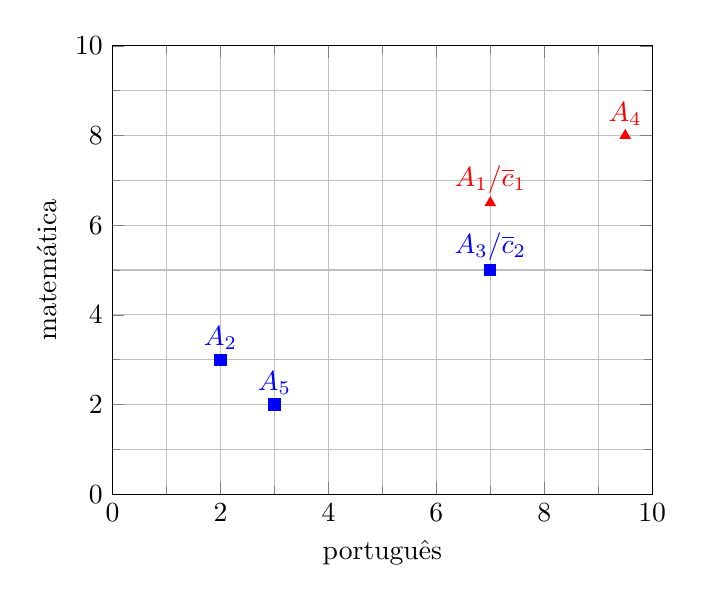
\begin{tikzpicture}
	\begin{axis}[
	grid=both,
	xmin=0, xmax=10,
	ymin=0, ymax=10,
	minor tick num = 1,
	nodes near coords,
	xlabel=português,
	ylabel=matemática
	]
	
	\addplot+[only marks, point meta=explicit symbolic, mark=triangle*]
	coordinates {
		(7, 6.5) [$A_1$/$\overline{c}_1$]
		(9.5, 8) [$A_4$]
	};
	
	\addplot+[only marks, point meta=explicit symbolic, mark=square*]
	coordinates {
		(7, 5) [$A_3$/$\overline{c}_2$]
		(2, 3) [$A_2$]
		(3, 2) [$A_5$]
	};
	\end{axis}
	\end{tikzpicture}
	
	\caption{Representação gráfica das notas dos alunos com alocação inicial}
	\label{fig:dados-notas-alunos-primeira-alocacao}
\end{figure}

O próximo passo consiste em recalcular os centroides em função dos elementos alocados a cada \textit{cluster}. O centroide será posicionado no valor médio dos atributos dos elementos. Como temos dois atributos, recalculamos os centroides como:

\begin{align*}
{\overline{c}_1}_1 &= ({A_1}_1 + {A_4}_1)/2 = (7,0 + 9,5)/2 = 8,25 \\
{\overline{c}_1}_2 &= ({A_1}_2 + {A_4}_2)/2 = (6,5 + 8,0)/2 = 7,25 \\
{\overline{c}_2}_1 &= ({A_2}_1 + {A_3}_1 + {A_5}_1)/3 = (2,0 + 7,0 + 3,0)/3 = 4,0 \\
{\overline{c}_2}_2 &= ({A_2}_2 + {A_3}_2 + {A_5}_2)/3 = (3,0 + 5,0 + 2,0)/3 = 3,3
\end{align*}

Logo, $\overline{c}_1 = (8,25; 7,25)$ e $\overline{c}_2 = (4,0; 3,3)$. A Figura~\ref{fig:dados-notas-alunos-novos-centroides} apresenta o conjunto de dados com os novos centroides (os centroides estão apresentados com o símbolo $\times$). Perceba que os centroides são posicionados no valor médio dos elementos do \textit{cluster}.

\begin{figure}[h]
	\centering
	\pgfplotsset{cycle list={red\\blue\\red\\blue\\}}
	
	
	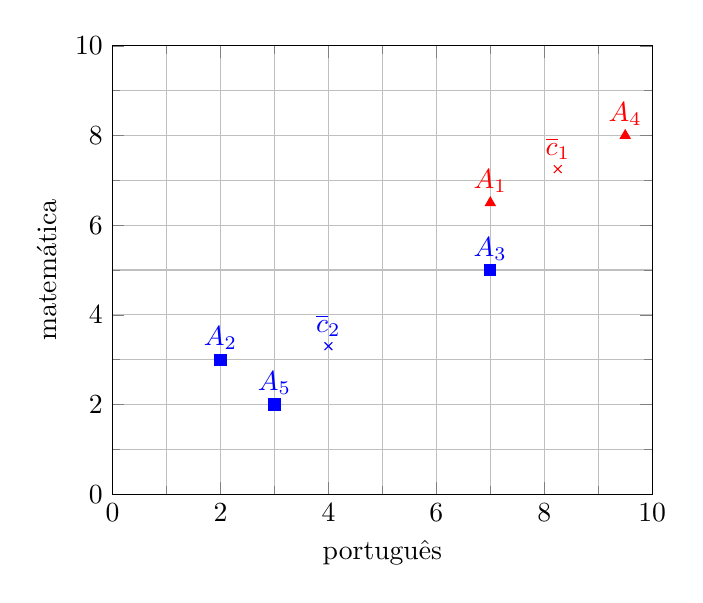
\begin{tikzpicture}
	\begin{axis}[
	grid=both,
	xmin=0, xmax=10,
	ymin=0, ymax=10,
	minor tick num = 1,
	nodes near coords,
	xlabel=português,
	ylabel=matemática
	]
	
	\addplot+[only marks, point meta=explicit symbolic, mark=x]
		coordinates {
			(8.25, 7.25) [$\overline{c}_1$]
		};
	
	\addplot+[only marks, point meta=explicit symbolic, mark=x]
		coordinates {
			(4, 3.3) [$\overline{c}_2$]
		};
	
	\addplot+[only marks, point meta=explicit symbolic, mark=triangle*]
		coordinates {
			(7, 6.5) [$A_1$]
			(9.5, 8) [$A_4$]
		};
	
	\addplot+[only marks, point meta=explicit symbolic, mark=square*]
		coordinates {
			(7, 5) [$A_3$]
			(2, 3) [$A_2$]
			(3, 2) [$A_5$]
		};
	\end{axis}
	\end{tikzpicture}
	
	\caption{Representação gráfica das notas dos alunos com novos centroides}
	\label{fig:dados-notas-alunos-novos-centroides}
\end{figure}

Com novos centroides, o próximo passo consiste em calcular as novas distâncias entre cada elemento e cada centroide. A matriz de distâncias resultante é apresentada abaixo.

\insertspace

\begin{center}
	\begin{tabular}{cccccccc}
		& & $A_1$ & $A_2$ & $A_3$ & $A_4$ & $A_5$ & \\
		$\overline{c}_1$ & \multirow{2}{*}{$\Bigg[$} & 1,5 & 7,6 & 2,6 & 1,5 & 7,4 & \multirow{2}{*}{$\Bigg]$} \\
		\multicolumn{1}{l}{$\overline{c}_2$} & & 4,4 & 2,0 & 3,4 & 7,2 & 1,6 & 
	\end{tabular}
\end{center}

\insertspace

Perceba que o elemento $A_3$, que antes pertencia ao \textit{cluster} $\overline{c}_2$, possui menor distância ao novo centroide $\overline{c}_1$. Logo, ele será realocado para este \textit{cluster}. A realocação é apresentada na matriz de alocação abaixo e a nova distribuição é apresentada na Figura~\ref{fig:dados-notas-alunos-nova-alocacao}.

\insertspace

\begin{center}
	\begin{tabular}{cccccccc}
		& & $A_1$ & $A_2$ & $A_3$ & $A_4$ & $A_5$ & \\
		$\overline{c}_1$ & \multirow{2}{*}{$\Bigg[$} & 1 & 0 & 1 & 1 & 0 & \multirow{2}{*}{$\Bigg]$} \\
		\multicolumn{1}{l}{$\overline{c}_2$} & & 0 & 1 & 0 & 0 & 1 & 
	\end{tabular}
\end{center}

\insertspace

\begin{figure}[h]
	\centering
	\pgfplotsset{cycle list={red\\blue\\red\\blue\\}}
	
	
	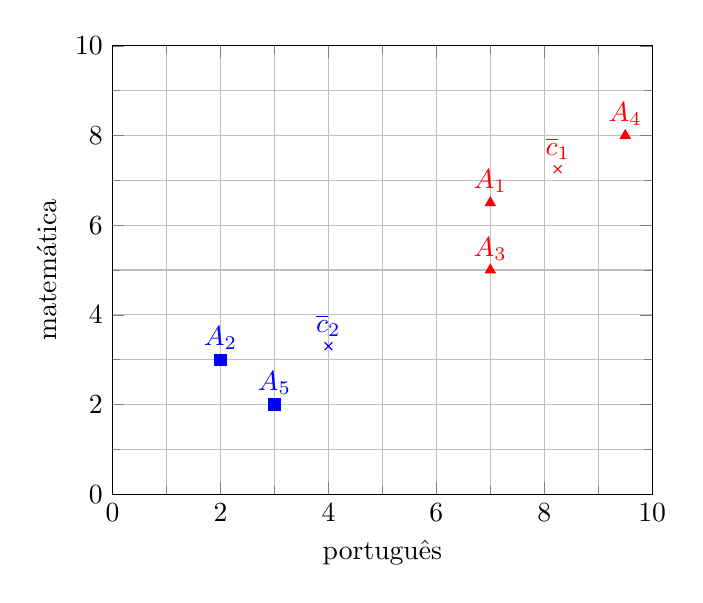
\begin{tikzpicture}
	\begin{axis}[
	grid=both,
	xmin=0, xmax=10,
	ymin=0, ymax=10,
	minor tick num = 1,
	nodes near coords,
	xlabel=português,
	ylabel=matemática
	]
	
	\addplot+[only marks, point meta=explicit symbolic, mark=x]
		coordinates {
			(8.25, 7.25) [$\overline{c}_1$]
		};
	
	\addplot+[only marks, point meta=explicit symbolic, mark=x]
		coordinates {
			(4, 3.3) [$\overline{c}_2$]
		};
	
	\addplot+[only marks, point meta=explicit symbolic, mark=triangle*]
		coordinates {
			(7, 6.5) [$A_1$]
			(7, 5) [$A_3$]
			(9.5, 8) [$A_4$]
		};
	
	\addplot+[only marks, point meta=explicit symbolic, mark=square*]
		coordinates {
			(2, 3) [$A_2$]
			(3, 2) [$A_5$]
		};
	\end{axis}
	\end{tikzpicture}
	
	\caption{Representação gráfica das notas dos alunos com a nova alocação}
	\label{fig:dados-notas-alunos-nova-alocacao}
\end{figure}

Como houveram mudanças de elementos entre os \textit{clusters}, os centroides devem ser recalculados. Os novos centroides são definidos por:

\begin{align*}
	{\overline{c}_1}_1 &= ({A_1}_1 + {A_3}_1 + {A_4}_1)/2 = (7,0 + 7,0 + 9,5)/3 = 7,8 \\
	{\overline{c}_1}_2 &= ({A_1}_2 + {A_3}_2 + {A_4}_2)/2 = (6,5 + 5,0 + 8,0)/3 = 6,5 \\
	{\overline{c}_2}_1 &= ({A_2}_1 + {A_5}_1)/3 = (2,0 + 3,0)/2 = 2,5 \\
	{\overline{c}_2}_2 &= ({A_2}_2 + {A_5}_2)/3 = (3,0 + 2,0)/2 = 2,5
\end{align*}

Os novos centroides são, portanto, $\overline{c}_1 = (7,8; 6,5)$ e $\overline{c}_2 = (2,5; 2,5)$. A Figura~\ref{fig:dados-notas-alunos-novos-centroides-2} apresenta os dados com os novos centroides. Novamente, os centroides são ajustados conforme a proximidade com os novos elementos dos \textit{clusters}.

\begin{figure}[h]
	\centering
	\pgfplotsset{cycle list={red\\blue\\red\\blue\\}}
	
	
	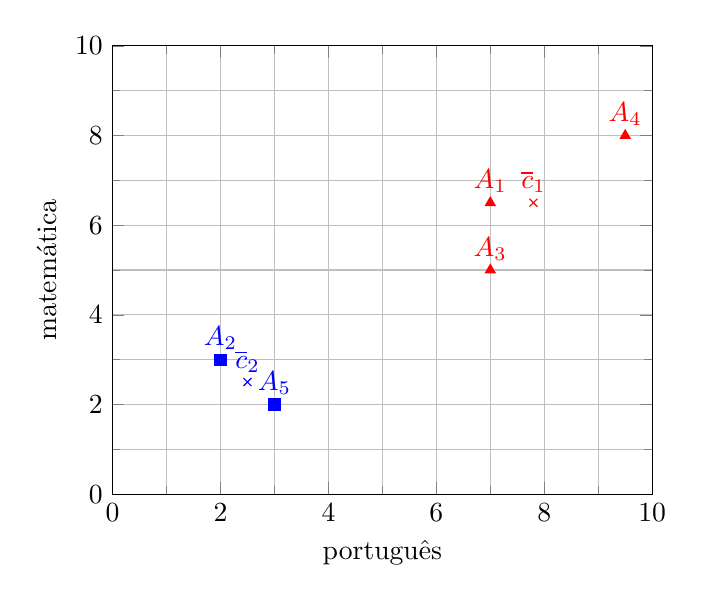
\begin{tikzpicture}
	\begin{axis}[
	grid=both,
	xmin=0, xmax=10,
	ymin=0, ymax=10,
	minor tick num = 1,
	nodes near coords,
	xlabel=português,
	ylabel=matemática
	]
	
	\addplot+[only marks, point meta=explicit symbolic, mark=x]
		coordinates {
			(7.8, 6.5) [$\overline{c}_1$]
		};
	
	\addplot+[only marks, point meta=explicit symbolic, mark=x]
		coordinates {
			(2.5, 2.5) [$\overline{c}_2$]
		};
	
	\addplot+[only marks, point meta=explicit symbolic, mark=triangle*]
		coordinates {
			(7, 6.5) [$A_1$]
			(7, 5) [$A_3$]
			(9.5, 8) [$A_4$]
		};
	
	\addplot+[only marks, point meta=explicit symbolic, mark=square*]
		coordinates {
			(2, 3) [$A_2$]
			(3, 2) [$A_5$]
		};
	\end{axis}
	\end{tikzpicture}
	
	\caption{Representação gráfica das notas dos alunos com novos centroides -- 2}
	\label{fig:dados-notas-alunos-novos-centroides-2}
\end{figure}

O próximo passo consiste em recalcular as distâncias entre cada elemento e cada novo centroide. A matriz de distâncias é dada por:

\insertspace

\begin{center}
	\begin{tabular}{cccccccc}
		& & $A_1$ & $A_2$ & $A_3$ & $A_4$ & $A_5$ & \\
		$\overline{c}_1$ & \multirow{2}{*}{$\Bigg[$} & 0,8 & 6,8 & 1,7 & 2,3 & 6,6 & \multirow{2}{*}{$\Bigg]$} \\
		\multicolumn{1}{l}{$\overline{c}_2$} & & 6,0 & 0,7 & 5,1 & 8,9 & 0,7 & 
	\end{tabular}
\end{center}

\insertspace

Com isso, a distribuição dos elementos aos \textit{cluster} fica a seguinte:

\insertspace

\begin{center}
	\begin{tabular}{cccccccc}
		& & $A_1$ & $A_2$ & $A_3$ & $A_4$ & $A_5$ & \\
		$\overline{c}_1$ & \multirow{2}{*}{$\Bigg[$} & 1 & 0 & 1 & 1 & 0 & \multirow{2}{*}{$\Bigg]$} \\
		\multicolumn{1}{l}{$\overline{c}_2$} & & 0 & 1 & 0 & 0 & 1 & 
	\end{tabular}
\end{center}

\insertspace

Como nenhum elemento trocou de \textit{cluster}, os centroides permanecem os mesmos e o algoritmo termina. Logo, o agrupamento final é aquele apresentado na Figura~\ref{fig:dados-notas-alunos-novos-centroides-2}. O primeiro \textit{cluster} é composto pelos elementos $\{A_1, A_3, A_4\}$, enquanto o segundo \textit{cluster} é composto pelos elementos $\{A_2, A_5\}$.

\section{Agrupamento hierárquico}

Os métodos de agrupamento hierárquicos também se baseiam na proximidade dos dados para execução da tarefa. Eles criam uma sequência de partições aninhadas, iniciando com cada elemento em um \textit{cluster} único e, iterativamente, une dois \textit{clusters} até formar um grande \textit{cluster} único. Cada partição intermediária é mantida e pode ser recuperada.

\subsection{Método aglomerativo}

O método aglomerativo é o algoritmo hierárquico de agrupamento mais utilizado. Seu pseudocódigo é apresentado no Algoritmo~\ref{alg:metodo-aglomerativo}. Considerando o tamanho do conjunto de dados $|X| = n$, criamos $n$ \textit{clusters}, cada um com um único elemento. A cada iteração, selecionamos os dois \textit{clusters} mais próximos e combinamos em um \textit{cluster} único. O algoritmo termina quando todos os elementos pertencem ao mesmo \textit{cluster}.

\begin{algorithm}[h]
	\DontPrintSemicolon
	\Entrada{\textit{conjunto de dados -- $X$}}
	\Saida{\textit{hierarquia de partições de $X$}}
	
	\Inicio{
		Criar $|X|$ \textit{clusters} e alocar cada objeto a um \textit{cluster}\;
		\Enqto{há clusters para agrupar}{
			Calcular matriz de distâncias entre os pares de \textit{clusters} disponíveis, utilizando uma \textit{\underline{métrica de integração}}\;
			Combinar o par de \textit{clusters} $c_i$ e $c_j$ mais próximo, gerando um único \textit{cluster} $c_{ij}$\;
		}
	}
	
	\caption{Pseudocódigo para o método aglomerativo de agrupamento hierárquico}
	\label{alg:metodo-aglomerativo}
\end{algorithm}

O resultado do método aglomerativo é toda a sequência de \textit{clusters} gerada durante a execução do algoritmo. Esta sequência pode ser analisada na forma de um dendrograma, como mostra a Figura~\ref{fig:exemplo-dendrograma}. O início do algoritmo apresenta todos os elementos separados em $n$ \textit{clusters} (base da imagem da esquerda). Na primeira iteração, os \textit{clusters} dos elementos $D$ e $E$ são combinados. Na segunda iteração, o \textit{cluster} $\{D, E\}$ é combinado com o \textit{cluster} do elemento $C$. Na terceira iteração, os \textit{clusters} dos elementos $A$ e $B$ são combinados. A execução segue até que todos os elementos estejam combinados em um elemento único. As uniões do dendrograma mostram a hierarquia dos \textit{clusters}, quanto mais acima, mais geral é o \textit{cluster}.

\begin{figure}[h]
	\centering
	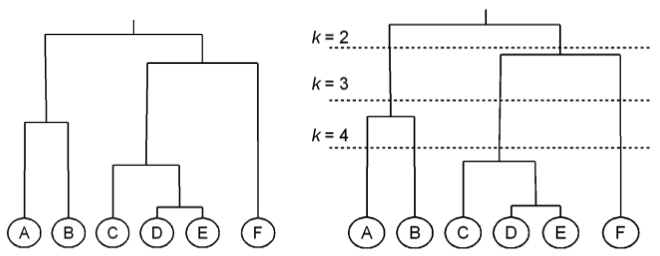
\includegraphics[width=\textwidth]{img/exemplo-dendrograma}
	\caption{Exemplo de dendrograma resultante do método aglomerativo}
	\label{fig:exemplo-dendrograma}
\end{figure}

Dada a hierarquia gerada, é possível recuperar o número desejado de \textit{clusters}. Isso é apresentado na imagem da direita da Figura~\ref{fig:exemplo-dendrograma}. Caso queiramos obter 4 \textit{clusters}, é realizado um corte no dendrograma com o número de partições correspondente. Ou seja, é possível recuperar qualquer quantidade de \textit{clusters}. Por exemplo, os \textit{clusters} resultantes para diferentes valores de $k$ são:
\begin{itemize}
	\item $k = 2$: $\{A, B\}$ e $\{C, D, E, F\}$.
	\item $k = 3$: $\{A, B\}$, $\{C, D, E\}$ e $\{F\}$.
	\item $k = 4$: $\{A\}$, $\{B\}$, $\{C, D, E\}$ e $\{F\}$.
\end{itemize}

Para implementar o método aglomerativo, é necessário definir a \textbf{métrica de integração} utilizada para calcular a distância entre diferentes \textit{clusters}. Existem quatro principais abordagens: ligação mínima, ligação máxima, ligação média e centroide. Estas abordagens são ilustradas na Figura~\ref{fig:exemplos-distancias-cluster}.

\begin{figure}[h]
	\centering
	
	\subfigure[]{
		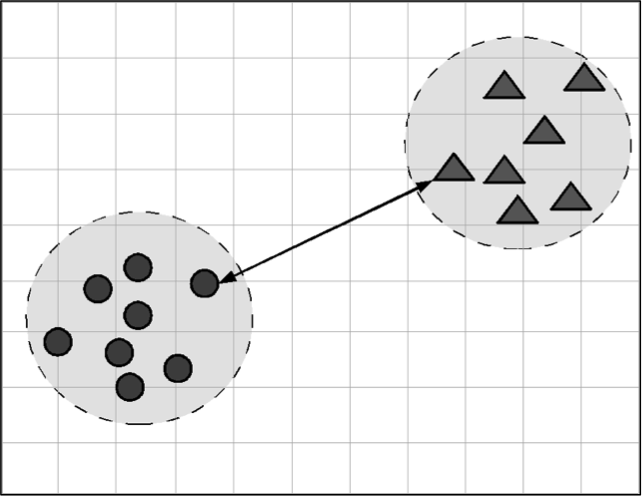
\includegraphics[width=0.4\textwidth]{img/dist-ligacao-minima}
	}
	\subfigure[]{
		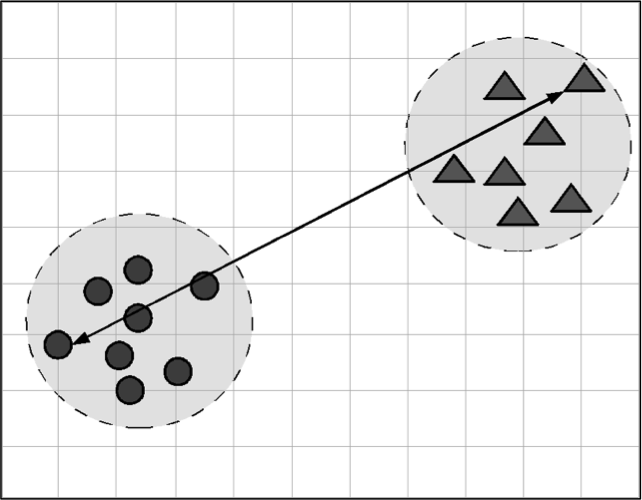
\includegraphics[width=0.4\textwidth]{img/dist-ligacao-maxima}
	}
	\subfigure[]{
		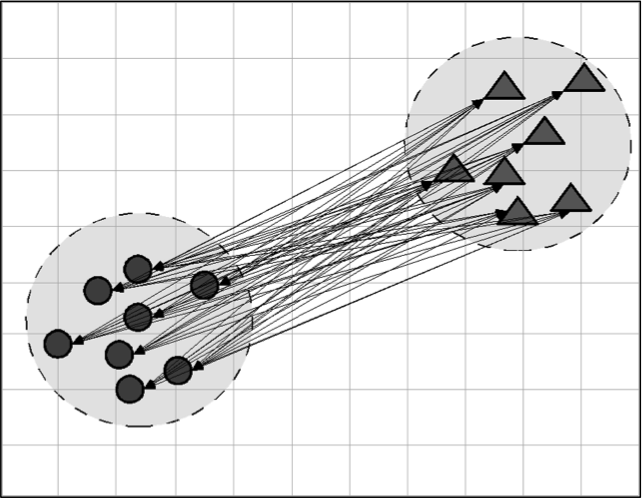
\includegraphics[width=0.4\textwidth]{img/dist-ligacao-media}
	}
	\subfigure[]{
		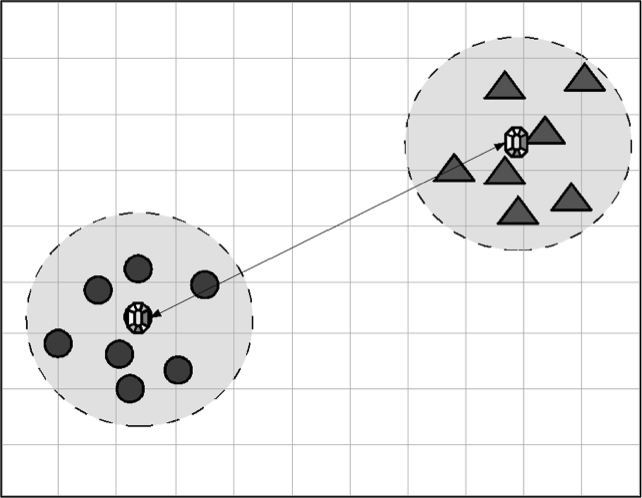
\includegraphics[width=0.4\textwidth]{img/dist-centroide}
	}
	
	\caption{Métricas de integração (distâncias) entre \textit{clusters}}
	\label{fig:exemplos-distancias-cluster}
\end{figure}

A \textbf{ligação mínima} (Figura~\ref{fig:exemplos-distancias-cluster} -- \texttt{a}) utiliza como distância entre dois \textit{clusters} a distância entre o par de elementos mais próximos de ambos. A \textbf{ligação máxima} (Figura~\ref{fig:exemplos-distancias-cluster} -- \texttt{b}) adota a estratégia oposta, utilizando a distância entre o par de elementos mais distantes em ambos os \textit{clusters}. A \textbf{ligação média} (Figura~\ref{fig:exemplos-distancias-cluster} -- \texttt{c}) calcula a distância entre todos os pares de elementos entre os \textit{clusters} e utiliza como média a métrica destes valores. Finalmente, a abordagem por \textbf{centroide} (Figura~\ref{fig:exemplos-distancias-cluster} -- \texttt{d}) calcula o centroide de cada \textit{cluster} e adota como métrica a distância entre eles.

O método aglomerativo é frequentemente utilizado pela sua flexibilidade com relação ao nível de granularidade, pela facilidade de adoção de diferentes métricas para a distância e pela possibilidade de utilizar atributos de diferentes naturezas. No entanto, esta abordagem possui um critério de terminação vago e não retorna para modificar \textit{clusters} já construídos. A complexidade do método é $O(n^2)$.

\subsection{Exemplo -- agrupamento hierárquico de alunos}

Vamos considerar o mesmo conjunto de dados da Seção~\ref{sec:exemplo-k-means}, com as notas obtidas pelos cinco alunos nas disciplinas de português e matemática. A Tabela~\ref{tab:dados-notas-alunos-2} apresenta novamente estes dados. A representação gráfica dos dados é reapresentada na Figura~\ref{fig:dados-notas-alunos-2}.

\begin{table}[h]
	\centering
	
	\begin{tabular}{lrr}
		\hline
		\textbf{Aluno} & \textbf{Português} & \textbf{Matemática} \\
		\hline
		$A_1$ & 7,0 & 6,5 \\
		$A_2$ & 2,0 & 3,0 \\
		$A_3$ & 7,0 & 5,0 \\
		$A_4$ & 9,5 & 8,0 \\
		$A_5$ & 3,0 & 2,0 \\
		\hline
	\end{tabular}
	
	\caption{Conjunto de dados das notas dos alunos}
	\label{tab:dados-notas-alunos-2}
\end{table}

\begin{figure}[h]
	\centering
	\pgfplotsset{cycle list={black}}
	
	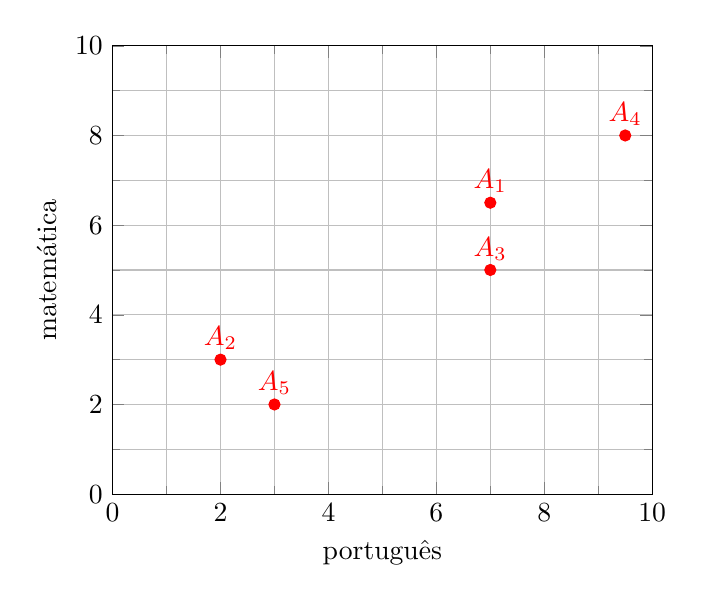
\begin{tikzpicture}
	\begin{axis}[
		grid=both,
		xmin=0, xmax=10,
		ymin=0, ymax=10,
		minor tick num = 1,
		nodes near coords,
		xlabel=português,
		ylabel=matemática
	]
	
	\addplot+[only marks, point meta=explicit symbolic, mark=*]
		coordinates {
			(7, 6.5) [$A_1$]
			(2, 3) [$A_2$]
			(7, 5) [$A_3$]
			(9.5, 8) [$A_4$]
			(3, 2) [$A_5$]
		};
	\end{axis}
	\end{tikzpicture}
	
	\caption{Representação gráfica das notas dos alunos}
	\label{fig:dados-notas-alunos-2}
\end{figure}

Cada elemento do conjunto de dados forma um \textit{cluster}. O primeiro passo consiste em calcular a distância entre cada \textit{cluster}. Adotaremos a ligação mínima entre \textit{clusters} como métrica de integração. Com isso, as distâncias são definidas como:

\insertspace

\begin{center}
	\begin{tabular}{cccccc}
		      & $A_1$ & $A_2$ & $A_3$ & $A_4$ & $A_5$ \\
		$A_1$ &   0   &  6,1  &  1,5  &  2,9  &  6,0  \\
		$A_2$ &   -   &   0   &  5,4  &  9,0  &  1,4  \\
		$A_3$ &   -   &   -   &   0   &  2,4  &  5,0  \\
		$A_4$ &   -   &   -   &   -   &   0   &  8,8  \\
		$A_5$ &   -   &   -   &   -   &   -   &   0
	\end{tabular}
\end{center}

\insertspace

Os elementos/\textit{clusters} mais próximos são $A_2$ e $A_5$. Logo, eles são selecionados para formar um único \textit{cluster}. A Figura~\ref{fig:dados-notas-alunos-particao} apresenta o conjunto de dados com a combinação dos elementos $A_2$ e $A_5$ em um único \textit{cluster}.

\begin{figure}[h]
	\centering
	\pgfplotsset{cycle list={black}}
	
	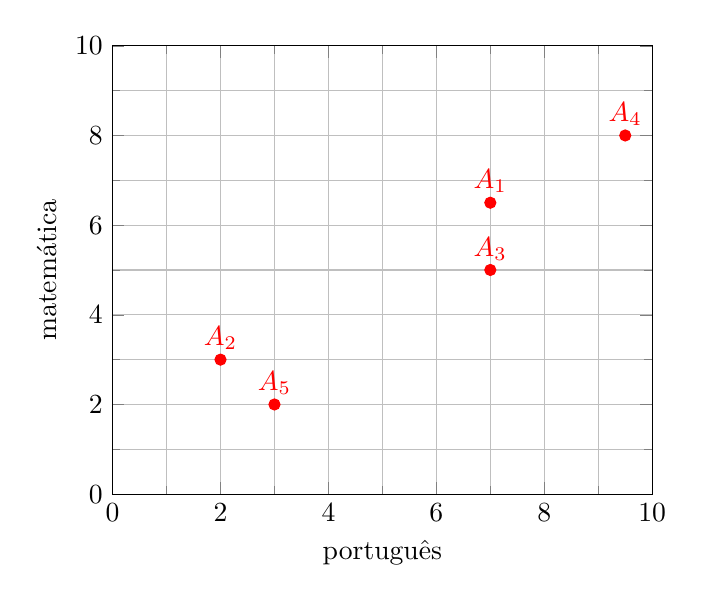
\begin{tikzpicture}
	\begin{axis}[
		grid=both,
		xmin=0, xmax=10,
		ymin=0, ymax=10,
		minor tick num = 1,
		nodes near coords,
		xlabel=português,
		ylabel=matemática
	]
	
	\addplot+[only marks, point meta=explicit symbolic, mark=*]
	coordinates {
		(7, 6.5) [$A_1$]
		(2, 3) [$A_2$]
		(7, 5) [$A_3$]
		(9.5, 8) [$A_4$]
		(3, 2) [$A_5$]
	};
	
	\draw [red] (26,28) ellipse [
		rotate=45,
		x radius=8,
		y radius=16,
	];
	
	\end{axis}
	\end{tikzpicture}
	
	\caption{Representação gráfica das notas dos alunos com a primeira combinação}
	\label{fig:dados-notas-alunos-particao}
\end{figure}

Ao recalcular as distâncias, devemos considerar os quatro \textit{clusters} existentes: $\{A_2, A_5\}$, $A_1$, $A,3$ e $A_4$. No cálculo da distância entre um elemento e o \textit{cluster} $\{A_2, A_5\}$, devemos considerar o elemento do \textit{cluster} mais próximo do segundo elemento (ligação mínima). Observando a Figura~\ref{fig:dados-notas-alunos-particao}, percebemos que os \textit{clusters} mais próximos são $\{A_1\}$ e $\{A_3\}$, que serão recombinados. Os \textit{clusters} da nova iteração são apresentados na Figura~\ref{fig:dados-notas-alunos-particao-2}.

\begin{figure}[h]
	\centering
	\pgfplotsset{cycle list={black}}
	
	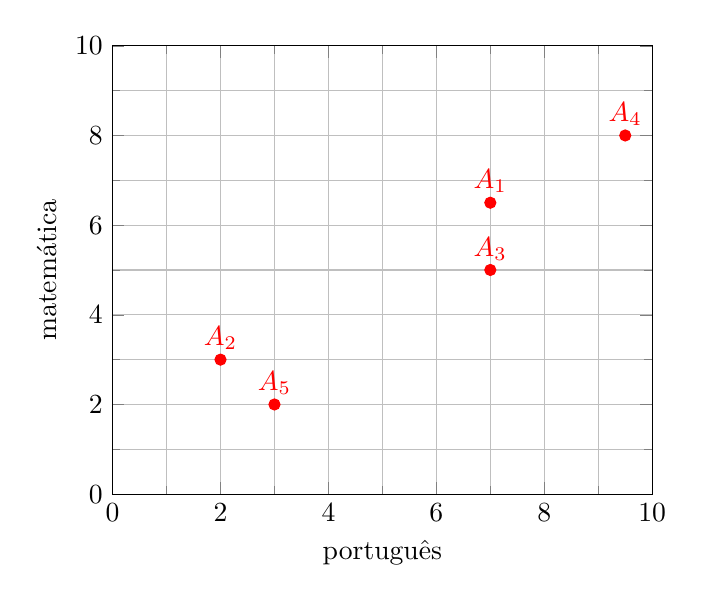
\begin{tikzpicture}
	\begin{axis}[
		grid=both,
		xmin=0, xmax=10,
		ymin=0, ymax=10,
		minor tick num = 1,
		nodes near coords,
		xlabel=português,
		ylabel=matemática
	]
	
	\addplot+[only marks, point meta=explicit symbolic, mark=*]
		coordinates {
			(7, 6.5) [$A_1$]
			(2, 3) [$A_2$]
			(7, 5) [$A_3$]
			(9.5, 8) [$A_4$]
			(3, 2) [$A_5$]
		};
	
	\draw [red] (26,28) ellipse [
		rotate=45,
		x radius=8,
		y radius=16,
	];
	
	\draw [blue] (70,60) ellipse [
		rotate=0,
		x radius=8,
		y radius=16,
	];
	
	\end{axis}
	\end{tikzpicture}
	
	\caption{Representação gráfica das notas dos alunos com a segunda combinação}
	\label{fig:dados-notas-alunos-particao-2}
\end{figure}

A próxima iteração seleciona os \textit{clusters} $\{A_1, A_3\}$ e $\{A_4\}$ para combinação, gerando a partição apresentada na Figura~\ref{fig:dados-notas-alunos-particao-3}. Finalmente, os dois \textit{clusters} são combinados, conforme apresentado na Figura~\ref{fig:dados-notas-alunos-particao-4}. O algoritmo finaliza sua execução, pois criou toda a hierarquia de \textit{clusters}.

\begin{figure}[h]
	\centering
	\pgfplotsset{cycle list={black}}
	
	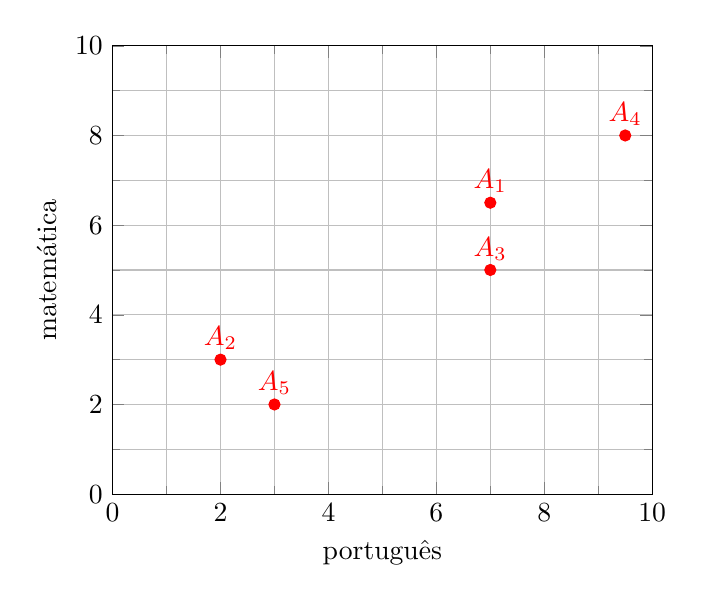
\begin{tikzpicture}
	\begin{axis}[
		grid=both,
		xmin=0, xmax=10,
		ymin=0, ymax=10,
		minor tick num = 1,
		nodes near coords,
		xlabel=português,
		ylabel=matemática
	]
	
	\addplot+[only marks, point meta=explicit symbolic, mark=*]
		coordinates {
			(7, 6.5) [$A_1$]
			(2, 3) [$A_2$]
			(7, 5) [$A_3$]
			(9.5, 8) [$A_4$]
			(3, 2) [$A_5$]
		};
	
	\draw [red] (26,28) ellipse [
		rotate=45,
		x radius=8,
		y radius=16,
	];
	
	\draw [blue] (70,60) ellipse [
		rotate=0,
		x radius=8,
		y radius=16,
	];
	
	\draw [green] (78,68) ellipse [
		rotate=315,
		x radius=16,
		y radius=30,
	];
	
	\end{axis}
	\end{tikzpicture}
	
	\caption{Representação gráfica das notas dos alunos com a terceira combinação}
	\label{fig:dados-notas-alunos-particao-3}
\end{figure}

\begin{figure}[h]
	\centering
	\pgfplotsset{cycle list={black}}
	
	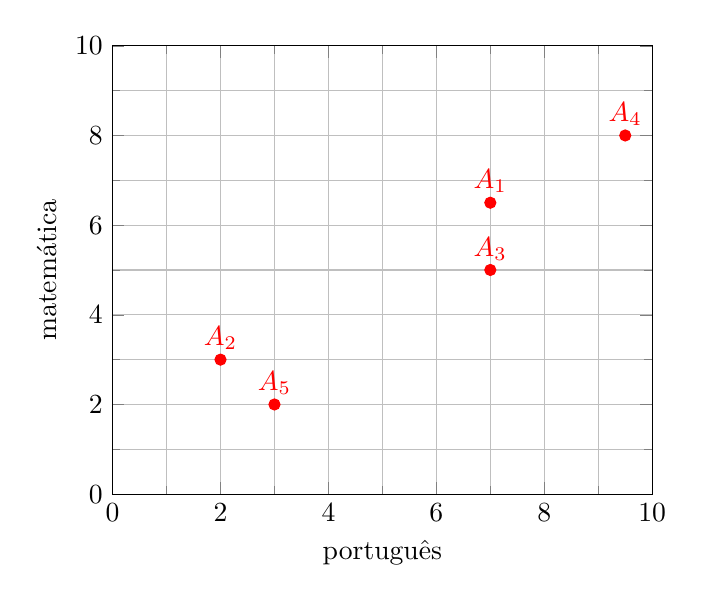
\begin{tikzpicture}
	\begin{axis}[
		grid=both,
		xmin=0, xmax=10,
		ymin=0, ymax=10,
		minor tick num = 1,
		nodes near coords,
		xlabel=português,
		ylabel=matemática
	]
	
	\addplot+[only marks, point meta=explicit symbolic, mark=*]
		coordinates {
			(7, 6.5) [$A_1$]
			(2, 3) [$A_2$]
			(7, 5) [$A_3$]
			(9.5, 8) [$A_4$]
			(3, 2) [$A_5$]
		};
	
	\draw [red] (26,28) ellipse [
		rotate=45,
		x radius=8,
		y radius=16,
	];
	
	\draw [blue] (70,60) ellipse [
		rotate=0,
		x radius=8,
		y radius=16,
	];
	
	\draw [green] (78,68) ellipse [
		rotate=315,
		x radius=16,
		y radius=30,
	];
	
	\draw [brown] (56,55) ellipse [
		rotate=304,
		x radius=25,
		y radius=60,
	];
	
	\end{axis}
	\end{tikzpicture}
	
	\caption{Representação gráfica das notas dos alunos com a quarta combinação}
	\label{fig:dados-notas-alunos-particao-4}
\end{figure}

O resultado do método aglomerativo com as notas dos alunos pode (e deve) ser representado através de um dendrograma. Ele é capaz de apresentar a hierarquia de \textit{clusters} e facilita a recuperação deles conforme o número de \textit{clusters} desejado. A Figura~\ref{fig:dados-notas-alunos-dendrograma} apresenta o dendrograma resultante. Finalmente, podemos obter os \textit{clusters} de acordo com o valor desejado para $k$ (número de \textit{clusters}):
\begin{itemize}
	\item $k = 2$: $\{A_1, A_3, A_4\}$ e $\{A_2, A_5\}$.
	\item $k = 3$: $\{A_1, A_3\}$, $\{A_4\}$ e $\{A_2, A_5\}$.
	\item $k = 4$: $\{A_1\}$, $\{A_3\}$, $\{A_4\}$ e $\{A_2, A_5\}$.
\end{itemize}

\begin{figure}[h!]
	\centering
	
	\begin{tikzpicture}[sloped]
		\node (a1) at (-4,0) {$A_1$};
		\node (a3) at (-2,0) {$A_3$};
		\node (a4) at (0,0) {$A_4$};
		\node (a2) at (2,0) {$A_2$};
		\node (a5) at (4,0) {$A_5$};
		
		\node (a2a5) at (3,1) {};
		\draw (a2) |- (a2a5.center);
		\draw (a5) |- (a2a5.center);
		
		\node (a1a3) at (-3,2) {};
		\draw (a1) |- (a1a3.center);
		\draw (a3) |- (a1a3.center);
		
		\node (a1a3a4) at (-1.5,3) {};
		\draw (a1a3.center) |- (a1a3a4.center);
		\draw (a4) |- (a1a3a4.center);
		
		\node (a1a3a4a2a5) at (0.75,4) {};
		\draw (a1a3a4.center) |- (a1a3a4a2a5.center);
		\draw (a2a5.center) |- (a1a3a4a2a5.center);
		
		\node (top) at (0.75,4.5) {};
		\draw (a1a3a4a2a5.center) |- (top.center);
	\end{tikzpicture}
	
	\caption{Dendrograma do agrupamento hierárquico das notas dos alunos}
	\label{fig:dados-notas-alunos-dendrograma}
\end{figure}

\section{Exercícios}

\resetexercisenumbering

\begin{exercise}
Pesquise aplicações de algoritmos de agrupamento. Destaque as técnicas utilizadas e os resultados obtidos.
\end{exercise}

\begin{exercise}
Pesquise casos onde o algoritmo de $K$-Means não apresenta bons resultados.
\end{exercise}

\begin{exercise}
Pesquise sobre o algoritmo de agrupamento \textit{DBScan}. Como ele funciona quais suas vantagens em relação ao $K$-Means?
\end{exercise}

\begin{exercise}
Dados os três objetos apresentados abaixo (atributos de funcionários), calcule a distância entre cada par de elementos e mostre os dois elementos mais próximos.

\begin{table}[h]
	\centering
	\begin{tabular}{ccccc}
		\hline
		\textbf{Idade} & \textbf{Gênero} & \textbf{Tempo de serviço} & \textbf{Formação} & \textbf{Salário} \\ \hline
		24 & feminino  & 2                &   pós-graduação &         3.200,00         \\ 
		38 & masculino  & 12                &   superior &         4.800,00         \\
		29 & feminino  & 5                &   médio &         2.600,00         \\
		\hline
	\end{tabular}
\end{table}
\end{exercise}

\begin{exercise}
O dendrograma abaixo mostra o agrupamento hierárquico de marcas de veículos. Mostre os elementos de cada grupo, considerando diferentes quantidades de grupos: 2, 3 e 4.

\begin{figure}[h!]
	\centering
	
	\begin{tikzpicture}[sloped]
	\node (a1) at (-4,0) {VW};
	\node (a3) at (-2,0) {GM};
	\node (a4) at (0,0) {Honda};
	\node (a2) at (2,0) {BMW};
	\node (a5) at (4,0) {Audi};
	
	\node (a2a5) at (3,1) {};
	\draw (a2) |- (a2a5.center);
	\draw (a5) |- (a2a5.center);
	
	\node (a1a3) at (-3,2) {};
	\draw (a1) |- (a1a3.center);
	\draw (a3) |- (a1a3.center);
	
	\node (a1a3a4) at (-1.5,3) {};
	\draw (a1a3.center) |- (a1a3a4.center);
	\draw (a4) |- (a1a3a4.center);
	
	\node (a1a3a4a2a5) at (0.75,4) {};
	\draw (a1a3a4.center) |- (a1a3a4a2a5.center);
	\draw (a2a5.center) |- (a1a3a4a2a5.center);
	
	\node (top) at (0.75,4.5) {};
	\draw (a1a3a4a2a5.center) |- (top.center);
	\end{tikzpicture}
\end{figure}
\end{exercise}

\begin{exercise}
Considere parte do conjunto de dados das espécies de íris apresentada abaixo. Mostre a execução do algoritmo $K$-Means com $k = 3$ e apresente os três grupos resultantes. Mostre o resultado final em planos cartesianos para visualização dos elementos, elipses e grupos (o atributo espécie não deve ser utilizado).

\begin{table}[h]
	\centering
	\begin{tabular}{rrrrl}
		\hline
		\textbf{Comp. (P)} & \textbf{Larg. (P)} & \textbf{Comp. (S)} & \textbf{Larg. (S)} & \textbf{Espécie} \\
		\hline
		5,1 & 3,5 & 1,4 & 0,2 & Setosa \\
		4,9 & 3,0 & 1,4 & 0,2 & Setosa \\
		7,0 & 3,2 & 4,7 & 1,4 & Versicolor \\
		6,4 & 3,2 & 4,5 & 1,5 & Versicolor \\
		6,3 & 3,3 & 6,0 & 2,5 & Virgínica \\
		5,8 & 2,7 & 5,1 & 1,9 & Virgínica \\
		\hline
	\end{tabular}
\end{table}
\end{exercise}

\begin{exercise}
Considere os mesmos dados do exercício anterior. Mostre a execução do algoritmo aglomerativo de agrupamento hierárquico e apresente o dendrograma resultante.
\end{exercise}

\begin{exercise}
Considere os dados com as características de esponjas marinhas disponível em \url{https://archive.ics.uci.edu/ml/datasets/Sponge}. Utilize a ferramenta Weka para o agrupamento destes dados. Teste diferentes algoritmos de agrupamento e seus parâmetros. Verifique as métricas de avaliação proporcionadas pela ferramenta e analise o desempenho de cada algoritmo.
\end{exercise}

\begin{exercise}
Considere o mesmo conjunto de dados do exercício anterior. Utilize a biblioteca \textit{JavaML} (ou outra da sua escolha) para execução e avaliação dos algoritmos de agrupamento. Compare o desempenho com aqueles implementados na ferramenta Weka.
\end{exercise}

\begin{exercise}
Implemente o algoritmo de $K$-Means para o conjunto de 100 pontos abaixo. Mostre o valor dos centroides ao final da execução, a disposição dos pontos nos grupos e a representação cartesiana dos resultados.

\begin{table}[h]
	\centering
	\def\arraystretch{1}
	\resizebox{\textwidth}{!}{%
	\begin{tabular}{rr|rr|rr|rr|rr}
		\hline
		\textbf{x} & \textbf{y} & \textbf{x} & \textbf{y} & \textbf{x} & \textbf{y} & \textbf{x} & \textbf{y} & \textbf{x} & \textbf{y} \\ \hline
		2.9986 & 5.4115 	&	7.3792 & 5.6468 	&	2.2180 & 1.7299 	&	6.4154 & 5.4805 	&	8.7612 & 6.4911 	\\
		8.1588 & 4.9327 	&	7.7253 & 6.2002 	&	6.1123 & 5.3547 	&	6.7577 & 5.8193 	&	8.7992 & 6.4291 	\\
		-0.1911 & -1.7320 	&	11.1470 & 7.7087 	&	2.4562 & 3.5604 	&	7.3953 & 5.6697 	&	-1.5520 & -3.9206 	\\
		9.1571 & 6.2303 	&	1.8570 & 2.1072 	&	1.3797 & 0.3961 	&	9.5569 & 7.2170 	&	8.1765 & 6.0644 	\\
		0.8224 & -1.1243 	&	2.9573 & 3.7049 	&	3.2149 & 3.3001 	&	5.9958 & 4.5021 	&	6.8398 & 5.1538 	\\
		0.1308 & -1.8648 	&	0.8489 & 0.2223 	&	9.0940 & 7.0498 	&	8.2078 & 6.2118 	&	0.4978 & 0.4194 	\\
		8.7121 & 6.1395 	&	1.8367 & 1.5076 	&	2.3842 & 2.6039 	&	11.9082 & 7.6112 	&	6.0912 & 4.3148 	\\
		2.2625 & 3.1703 	&	4.7384 & 5.1813 	&	3.3281 & 5.1815 	&	6.0547 & 7.2849 	&	7.3719 & 5.9768 	\\
		1.7972 & 1.7397 	&	1.3665 & 0.6363 	&	8.8959 & 6.4742 	&	8.1267 & 7.0309 	&	8.4350 & 6.3067 	\\
		3.0634 & 3.0133 	&	10.5466 & 6.5951 	&	0.1479 & -0.6412 	&	5.3031 & 4.6593 	&	8.2206 & 6.7469 	\\
		8.1291 & 5.9392 	&	1.6342 & 2.1033 	&	3.0903 & 3.3168 	&	1.4604 & 1.1574 	&	8.2105 & 5.5732 	\\
		10.8097 & 6.8504 	&	6.5543 & 6.2060 	&	0.5014 & -0.0152 	&	10.4773 & 6.5726 	&	8.6842 & 6.3063 	\\
		0.6106 & 0.7215 	&	7.4471 & 6.0770 	&	4.3224 & 5.3156 	&	3.9189 & 4.9542 	&	7.2223 & 5.7820 	\\
		6.1466 & 5.7468 	&	8.0574 & 6.1558 	&	7.1978 & 5.5789 	&	1.1550 & 0.6860 	&	3.0846 & 1.4112 	\\
		6.3625 & 5.1882 	&	8.0896 & 6.3030 	&	7.8588 & 6.7083 	&	0.2094 & -1.9528 	&	6.6620 & 5.3358 	\\
		-1.6208 & -3.8387 	&	1.3350 & 0.4894 	&	9.0953 & 7.3278 	&	7.7698 & 4.9409 	&	4.1014 & 5.9718 	\\
		1.6859 & 1.6659 	&	3.1120 & 3.3676 	&	4.2530 & 5.6024 	&	5.5875 & 5.2593 	&	2.8341 & 4.9589 	\\
		3.8979 & 5.4510 	&	1.0531 & 1.6620 	&	9.4268 & 6.8458 	&	5.7082 & 4.2622 	&	7.8170 & 5.7399 	\\
		1.3537 & 0.7185 	&	1.7550 & 1.7793 	&	2.4428 & 2.1498 	&	2.5005 & 2.8861 	&	7.5139 & 6.1183 	\\
		1.2620 & 1.7233 	&	1.8914 & 0.7850 	&	9.0287 & 6.6842 	&	1.0037 & 0.3312 	&	2.1673 & 3.0574 	\\
		
		\hline
	\end{tabular}
	}
\end{table}
\end{exercise}